% manual for gs
% started december 2007
% andres.legarra@toulouse.inra.fr

% TODO
% put some "typical analysis" (BLUP, VCE, with or without SNP/animal effects)



\documentclass[a4paper,12pt,titlepage]{article}      % Specifies the document class
%\usepackage[dvips]{graphicx}
\usepackage{amsmath}
\usepackage[ansinew]{inputenc}
\usepackage{verbatim}
\usepackage{breakcites} %not to break citations
\usepackage{titlepic} %http://typethinker.blogspot.com/2008/08/picture-on-title-page-in-latex.html
\usepackage[pdftex]{color,graphicx} % this works only for pdflatex
\usepackage[pdftex]{hyperref} % this works only for pdflatex

\newcommand{\bsr}{\mathbf} %bold symbol, roman
\newcommand{\bsi}{\boldsymbol} %bold symbol, italic
\newcommand{\tm}{\texttt} %tipo maquina ;-)
                             % The preamble begins here.
                             
\title{\textsc{ {\Huge GS3} \\ 
{\normalsize Genomic Selection --- Gibbs Sampling --- Gauss Seidel  \\
(and BayesC$\pi$) }
}
%\footnote{ This program has been partially financed by FEDER European funds through POCTEFA: \url{http://www.poctefa.eu/}. }
}  % Declares the document's title.



\author{
	Andr\'es Legarra \thanks{\ttfamily andres.legarra [at] toulouse.inra.fr }
										\thanks{INRA, UR 631, F-31326 Auzeville, France }      
	\and Anne Ricard \thanks{\ttfamily anne.ricard [at] toulouse.inra.fr }
										\thanks{        INRA, UMR 1313, 78352 Jouy-en-Josas, France }
	\and Olivier Filangi \thanks{\ttfamily olivier.filangi [at] rennes.inra.fr }
												\thanks{INRA, UMR 598 35042 Rennes, France }
}
%\date{September 11, 2006}      % Deleting this command produces today's date.



%como meto un dibujito aqui?
\titlepic{
%\includegraphics[width=0.5\textwidth]{combined.jpg}
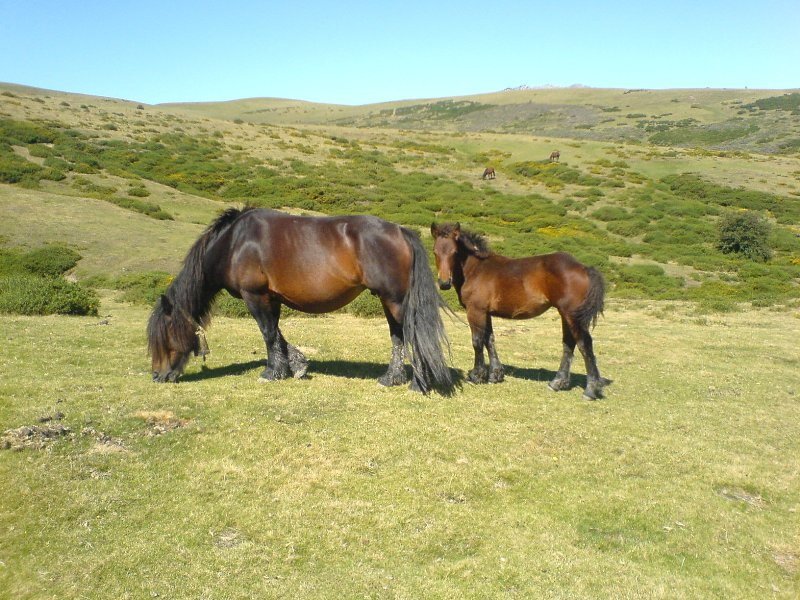
\includegraphics[width=0.5\textwidth]{DSC00130_petit.jpg}
}


\newcommand{\p}{p \,} 

\begin{document}             % End of preamble and beginning of text.

\maketitle                   % Produces the title.

\newpage
{\large
This program has been partially financed by FEDER European funds through POCTEFA: \url{http://www.poctefa.eu/}. }

\includegraphics[width=0.5\textwidth]{logo_cooperaci_n_01.jpg}

\includegraphics[width=0.5\textwidth]{logo_europa_fondos_feder_01.jpg}
and ANR project Rules \& Tools.

\newpage

%%\section{\huge 2 do}
%%
%%\begin{enumerate}
%%  \item missing esta hecho
%%	\item BayesC -> bibliografia
%%	\item BayesFactors
%%	\item Mixture option
%%	\item simulation option
%%	\item OPTION SEEDS
%%\end{enumerate}



{\footnotesize
\begin{verbatim}

Copyright (C) 2010  A Legarra, A Ricard, O Filangi

This program is free software: you can redistribute it and/or modify
it under the terms of the GNU General Public License as published by
the Free Software Foundation, either version 3 of the License, or
(at your option) any later version.

This program is distributed in the hope that it will be useful,
but WITHOUT ANY WARRANTY; without even the implied warranty of
MERCHANTABILITY or FITNESS FOR A PARTICULAR PURPOSE.  See the
GNU General Public License for more details.

You should have received a copy of the GNU General Public License
along with this program.  If not, see <http://www.gnu.org/licenses/>.
\end{verbatim}
}

\newpage
\tableofcontents
\newpage

\section{Introduction}      % Produces section heading.  Lower-level
                             % sections are begun with similar 
                             % \subsection and \subsubsection commands.

This draft describes using and understanding a software for genome-wide genetic evaluations and validations, inspired in the theory by \cite{Meuwissen2001a}, and used for own our research in \cite{Legarra2008a}.

In short: it estimates effects of SNPs, either using a priori normal distributions (GBLUP), or the Bayesian Lasso \cite{tibshirani1996regression,Campos2009a,Legarra2011} or a mixture of $\pi$ normal and $1-\pi$ a mass point at 0, namely BayesC(Pi) \cite{Kizilkaya2010,Fernando2010}. \emph{Note that our definition of $\pi$ here is {\large opposite} to those authors: $\pi=$ the fraction of SNPs ``having'' an effect.}


The program is self-contained, using modules from Ignacy Misztal's BLUPF90 distribution at \url{http://nce.ads.uga.edu/~ignacy}. Some functions and subroutines have been taken from the Alan Miller web page at  \url{http://users.bigpond.net.au/amiller/}. It has been tested with  NAG f95, ifort and gfortran $>=4.3$. Gustavo de los Campos helped us with the heterogenous variances and an R code for the Bayesian Lasso.

The computing methods have been described in \cite{Legarra2008}, as well as in \cite{Fernando2010}. 

\subsection{History}

We wrote this program to implement genome-wide genetic evaluation (\emph{aka} genomic selection) in mice \cite{Legarra2008a}, as there was nothing available around. The program uses Gibbs sampling, by means of an unconventional Gibbs sampling scheme \cite{Legarra2008}. It accepts quite general models.

We added BayesCPi end 2010, motivated basically for GWAS; and Bayesian Lasso in August 2011 as our previous version was not very user-friendly.

\section{Background}
Recently, the availability of massive ``cheap'' marker genotyping raised up the question on how to use these data for genetic evaluation and marker assisted selection. Proposals by \cite{Lande1990, Meuwissen2001a} among others, use a linear model for this purpose, in which each marker variant across the genome is assigned a linear effect, as follows:
$$ y_i = \sum_{j=1}^{n} \left( z_{ijk} a_{jk}  \right) + e_i $$
  
where $y_i$ is the phenotype of the $i$-th animal, $z_{ijk}$ is an indicator covariate for the $i$-th animal and the $j$-th marker locus in its $k$-th allelic form, and $e_i$ is a residual term. 
%This implies that for 10000 loci and biallelic markers, 20000 effects have to be estimated.
Hereinafter and for the sake of clarity we will refer to $a_{jk}$ as \emph{``marker locus effects''}. 

For the sake of simplicity, we further assumed biallelic loci and a simpler model as follows.
In the $j$-th locus, there are two possible alleles for each SNP (say a and A), and there are three possible genotypes: ``aa'', ``aA'' and ``AA''. We arbitrarily assign the value $ - \frac{1}{2}a_j$  to the allele ``a'' and the value $ + \frac{1}{2}a_j$ to the allele ``A'' \footnote{Convention for sign of $a$ has changed to the opposite as of 19/02/2013 (version 2.2.3). This generates an incompatibility backwards: solutions ofr additive SNP effects have signs reversed. EBVs, variances, and other efefcts keep unchanged.} This follows a classical parameterization in which $a_j$ is half the difference between the two homozygotes \cite{Lynch1998}. These are the additive effects of the SNP's and they can be thought of as classical substitution effects in the infinitesimal model. 

As for the dominant effect $d_j$, it comes up when the genotype is ``aA''.


\section{Models}


\subsection{General model}

The following kind of linear models is supported:

\begin{equation} \label{eq:SNPanimal}
 \bsr{y} = \bsr{X}\bsr{b} + \bsr{Za} + \bsr{Wd} + \bsr{Tg} + \bsr{Sp} + \bsr{e} 
\end{equation}

Including any number and kind (cross-classified, covariates) fixed effects ($\bsr{b}$), and random (multivariate normal) additive $\bsr{a}$ and dominant $\bsr{d}$ marker locus effects, polygenic infinitesimal effects $\bsr{g}$, and random environmental effects $\bsr{p}$ (also known as permanent effects).

 If the prior distribution of $\bsr{a}$ is considered to be normal \cite{VanRaden11012008}, this model is often called GBLUP or BLUP\_SNP. Random effects have associated variance components. You can estimate them using the software, or (much faster), if you have previous estimates of genetic variance $\sigma_u^2$, you can use an \emph{approximate} formula which is extensively discussed in \cite{Gianola2009a}:
$\sigma_a^2 = \sigma_u^2 / 2 \sum{p_i q_i}$
where $p_i$ is the allelic frequency at SNP $i$. 




%This is equal to the former model with the constraint $a_{j1}=a_{j2}$, which is implicit in BLUP for random effects (\cite{searle1997brb}).


\subsection{Heterogeneity of variances}


Heterogeneity of variances in the residual is accepted (v.gr., for use of DYD's with their accuracies) through a column of weights. These works as follows: let $\omega_i$ be the weight for record $i$. These implies that the distribution for $y_i$ is:

$y_i|\cdots = N(\hat{y}_i, \sigma_e^2 / \omega_i  )$, where 
$\hat{y}_i = \bsr{x}_i\bsr{b} + \bsr{z}_i\bsr{a} + \bsr{w}_i\bsr{d} + \bsr{t}_i\bsr{u} + \bsr{s}_i\bsr{c} $.

Thus $\bsr{e} \sim N(0,\bsr{R})$, where $\bsr{R}_{i,i} = \sigma_e^2 / \omega_i $.

In a typical case, weights $\omega$ are reliabilities of DYD's expressed as ``equivalent daughter contributions''. 

\subsection{Submodels}


\emph{Any} submodel from the above can be used \emph{but} random effects can only be included once, e.g., there is no possibility of including two random environmental effects (say litter and herd-year-season). 


\subsection{Mixture (BayesCPi) modelling of marker locus effects}

It is reasonable to assume that most marker loci are \emph{not} in linkage disequilibrium with markers. A way of selecting a subset of them is by fixing a non-negligible \emph{a priori} probability of their effects to be zero. Method BayesB \cite{Meuwissen2001a} achieved this through variance components having values of zero. An alternative approach is to set up  an indicator variable ($\delta$) stating whether the marker has any effect (1) or not (0). That is, the model becomes:

$$ y_i = \text{other effects} + \sum_{j=1}^{n} \left( z_{ij} a_{j} \delta_{j}  \right) + e_i $$

with $\delta_j = (0,1)$. The distribution of $\bsi{\delta}=(\delta_1 \ldots \delta_n$) can be posited as a binomial, with probability $\pi$. This model (a mixture model) is more parsimonious than \cite{Meuwissen2001a} and MCMC is straightforward \cite{Fernando2010}. On the other hand a prior distribution has to be postulated for $\pi$, and this is a beta distribution. Details can be found in \cite{Kizilkaya2010}.

\subsection{Bayesian Lasso}

The Lasso (least absolute shrinkage and selection
operator \cite{tibshirani1996regression}) combines variable selection
and shrinkage. Its Bayesian counterpart, the
Bayesian Lasso \cite{park2008bl} provides a
more natural interpretation in terms of a priori distributions.
In particular, Bayesian Lasso provides a fully
parametric model with a simple Gibbs sampler implementation. Further, the exponential
distribution of the Lasso is thought to reflect
reasonably well the nature of quantitative trait
locus (QTL) effects \cite{Goddard2009a}. The Bayesian Lasso has been used in genomic selection with good results  \cite{Campos2009a,Legarra2011}.  There are two possible implementations of the Bayesian Lasso  \cite{tibshirani1996regression,park2008bl}; \cite{Legarra2011} compared both. In this program, only Tibshirani's implementation is used; this was called BL2Var by \cite{Legarra2011}. To use Park \& Casella 's \cite{park2008bl}, I recommend package BLR for R, available in 
\href{http://cran.r-project.org/web/packages/BLR/index.html}{http://cran.r-project.org/web/packages/BLR/index.html}.

For an individual SNP, the prior distribution is thus as follows:

$$\Pr(a_i |\lambda)=\frac{\lambda}{2} \exp(-\lambda |a_i |)$$

But this can be written as:

$$\Pr(a_i |\tau^2)=N(0,\tau_i^2)$$

$$\Pr(\tau^2_i)=\frac{\lambda^2}{2} \exp(-\lambda^2 |\tau_i^2 |)$$

So, basically we are estimating individual variances fo each SNP (as in BayesB). These variances can be used to weight each SNP when constructing a genomic relationship matrix.
Initial value for parameter $lambda$ is not entered as such; rather, an initial value of  $\lambda^2=2/\sigma^2_a$ is used.


\subsection{A priori information}

Prior inverted-chi squared distributions can be postulated for  variance components $\sigma^2_a$, $\sigma^2_d$, $\sigma^2_u$, $\sigma^2_c$, $\sigma^2_e$ for estimation with \verb|VCE|. These are also starting values.
For ease of use, we have considered that beta distributions (with $\alpha$ and $\beta$ parameters) for $\pi$ and inverted-chi squared distributions for the different variances. 
Note that values of $\alpha=0$ or $\beta=0$ will cause problems because the Beta distribution will be ill-defined. Note also that
\begin{itemize}
 \item \tm{$\alpha=1$ , $\beta=1$} $\rightarrow$ uniform distribution on $\pi$. 
 \item \tm{$\alpha=1$ , $\beta=10d10$} $\rightarrow$ $\pi$ almost certainly close to 0 (most SNPs have no effect).
 \item \tm{$\alpha=10d8$ , $\beta=10d10$} $\rightarrow$ $\pi$ almost exactly fixed to 0.01 (on average, 10\% SNPs will have an effect).
\end{itemize}


These prior distributions are used when a full MCMC is run but not for \verb|BLUP| estimation or in the \verb|PREDICT| option.

For $\lambda$ the prior is bounded between 0 and $10^7$.


\section{Functionality}

\subsection{MCMC}
A full MCMC is run with the keyword \verb|VCE|. This samples all possible unknowns  $(\bsr{y},\bsr{b},\bsr{a},\bsr{d},\bsr{g}, \bsr{p}, % \bsr{e},
 \sigma^2_a,\sigma^2_d,\sigma^2_g,\sigma^2_p,\sigma^2_e)$ 
 and $\bsi{\delta}$ and hyperparameter $\pi$ if requested
 . Output are samples of variance components components 
 and $\pi$ 
 and a posteriori means for $\bsr{b},\bsr{a},\bsr{d},\bsr{g}, \bsr{p}$. ``Generalized'' genomic breeding value estimates (EBV's) , i.e., the sum of the  ``polygenic'' (pedigree based) and the SNP effects: $EBV_i = \hat{g}_i + \bsr{z_i\hat{a}} + \bsr{z_i\hat{d}}$ are also in the output.

Continuation (in the case of sudden interruption or just the desire of running more iterations) are possible via a specific keyword (but not for the Bayesian Lasso). The continuation is done by reading the last saved state of the MCMC chain, so be careful not to delete that file (named \verb|parameter_file_cont|).

\subsection{BLUP}
BLUP is defined here in the spirit of Henderson's BLUP, as in \cite{Meuwissen2001a}. Therefore it is an estimator that assumes known variances for all random effects
and $\bsi{\delta} = \bsr{1},\pi=1$ (i.e. there is no filtering on which markers trace QTLs). 
The keyword is \verb|BLUP|.

\subsection{MCMCBLUP}
Same as before, but random effects are estimated via Gibbs sampler (assuming known variances). These provides standard errors of the estimates.
The keyword is \verb|MCMCBLUP|.

\subsubsection{Bayes Factors}
Here there is the way of computing Bayes Facyor from results of SNP-BLUP. Including at the end the option 
\begin{verbatim}
OPTION Bayes Factor n a b
\end{verbatim}

where (optional, with default value 1) $n$ indicates the number of consecutive markers (bracket) considered (e.g. Bayes Factors will be computed for sizes 1, then 2... up to $n$ ), and (optional, but if they are included $n$ must be explicitly indicated) $a$ and $b$ indicate the first and last marker to be included in the computations. Note that the larger the $n$ the more resources will be consumed. The output is on file  \mbox{\texttt{parameter file\_BF}}. with columns \verb|i pos nBF BF logp0 logp1|: number of the leftmost marker considered, number of the marker in the middle of the bracket, the \emph{log} (in natural base) of the Bayes Factor and its two components logL0 and logL1.

\subsection{PREDICT}
Option PREDICT computes estimates of the prediction of phenotype given model estimates. This is useful for cross-validation, but for computation of overall individual genetic values as well, if any of $\bsr{a},\bsr{d},\bsr{u}$ are included. Additive values would be $\bsr{a},\bsr{u}$. The keyword is \verb|PREDICT|.

For example, if you have candidates for selection, create a file with dummy phenotypes (e.g. 0) and pass them through \verb|PREDICT|.

\section{Use}

\subsection{Parameter file}
This is an example of a typical file running a full MCMC analysis. It is quite messy \verb| :-(|. Be careful, the order has to be kept!

{\small
\begin{verbatim}
DATAFILE
./exo_data.txt
PEDIGREE FILE
./pedigri.dat
GENOTYPE FILE
./exo_genotypes.txt
NUMBER OF LOCI (might be 0)
10946
METHOD (BLUP/MCMCBLUP/VCE/PREDICT)
VCE
SIMULATION
F
GIBBS SAMPLING PARAMETERS
NITER
10
BURNIN
2
THIN
10
CONV_CRIT (MEANINGFUL IF BLUP)
1d-4
CORRECTION (to avoid numerical problems)
1000
VARIANCE COMPONENTS SAMPLES
var2
SOLUTION FILE
solutions2
TRAIT AND WEIGHT COLUMNS
1 0 #weight
NUMBER OF EFFECTS
5
POSITION IN DATA FILE TYPE OF EFFECT  NUMBER OF LEVELS
6 cross 1
5 add_animal 2272
7 perm_diagonal 2000
8 add_SNP 0
8 dom_SNP 0
VARIANCE COMPONENTS (fixed for any BLUP, starting values for VCE)
vara
2.52d-04 2
vard
1.75d-06 2
varg
3.56 2
varp
2.15 2
vare
0.19 2
RECORD ID
5
CONTINUATION (T/F)
F
MODEL (T/F for each effect)
T T T T T
A PRIORI a
1 1
a PRIORI D
1 1
USE MIXTURE (BAYES C)
T
\end{verbatim}
}

Let analyze by \emph{logical} sections.

\subsubsection{Files and input-output}
This should be self-explanatory. If you do not have pedigree file, put a blank line.
\begin{verbatim}
DATAFILE
./exo.txt
PEDIGREE FILE
./pedigri.dat
GENOTYPE FILE
./exo_genotypes.txt
...
VARIANCE COMPONENTS SAMPLES
var.cage.animal.txt
SOLUTION FILE
solutions.cage.animal.txt
\end{verbatim}

Note that the continuation file is automatically created as \newline \mbox{\texttt{parameter file\_cont}}.

Other files automatically created are \mbox{\texttt{predictions}} (if \verb|PREDICT|) and 
\newline \mbox{\texttt{parameter file\_EBVs}} with estimated breeding values.

%The \verb|FORMAT| statement has to contain a valid Fortran format. Fixed format is needed in order to read the SNPs in a simple way. In the example, there are 7 columns with numbers (either integer or real) or width 12, one space, and a single, long, chain of characters of width 21892 (i.e. twice the number of SNPs).

\subsubsection{Model features}

\begin{verbatim}
NUMBER OF LOCI (might be 0)
10946
METHOD (BLUP/MCMCBLUP/VCE/PREDICT)
BLUP
...
TRAIT AND WEIGHT COLUMNS
1 0 #column 0 for weight means no weight
NUMBER OF EFFECTS
5
POSITION IN DATA FILE TYPE OF EFFECT  NUMBER OF LEVELS
6 cross 1
5 add_animal 2272
7 perm_diagonal 600
8 add_SNP 0
8 dom_SNP 0
...
MODEL (T/F for each effect)
T T T T T
...
USE MIXTURE (BAYESC)
T
\end{verbatim}




In the \texttt{TRAIT AND WEIGHT COLUMNS} the column of trait and its weight have to be specified.  If the column for weight is 0, then no weight is assumed.


For the methods, see above.
 
This is a model with one fixed effect (overall mean), 2272 polygenic (pedigree-based) random effects, 600 ``permanent'' effects and dominant and additive effects for the SNPs. The number of loci is the total number of SNPs, but this is again computed from the data file.

This section allows to describe your model and put or remove effects. { \Huge Remember: you need to put at least a ``fixed'' cross-classified effect, for instance an overall mean. This is not done automatically.} If you only fit random effects, you might get very, very weird results.

Write as many lines under \texttt{POSITION...} as number of effects. The \texttt{POSITION} means in which the column the effect is located in the data file (which has to be in free format, i.e., columns separated by spaces). This is irrelevant for \texttt{add\_SNP} and \texttt{dom\_SNP}, they are read from genotype file. The \tm{TYPE OF EFFECT} is one of the following (with their respective keywords):
\begin{itemize}
  \item   \texttt{ cross }
       generic cross-classified ''fixed'' effect
  \item  \texttt{ cov }
       generic covariable 
  \item     \texttt{ add\_SNP }
         additive SNP effect
  \item   \texttt{ dom\_SNP }
       dominant SNP effect
% not implemented yet
%  \item   \texttt{ ind\_SNP }
%       individual SNP effect
  \item   \texttt{ add\_animal }
       additive infinitesimal effect
   \item  \texttt{ (perm\_diagonal)}
       generic environmental random effect 
\end{itemize}
You can put in your model as many generic covariables and cross-classified ``fixed'' effects as you want but you can put \emph{only one} (or none) of the other. 

The \tm{NUMBER OF LEVELS} has to be 1 for covariables (no possibility for nested covariables and the like); for the SNP effects, it is determined by the \tm{NUMBER OF LOCI}.

The \tm{MODEL} statement allows to quickly change the model fixing a logical variable \tm{in\_model} to true (\tm{t}) or false (\tm{f}). But using this feature quickly becomes confusing.

The \tm{USE MIXTURE (BAYESC)} statement starts (if \tm{VCE}) 
the BayesCPi method.

\subsubsection{How to use the Bayesian Lasso}
This is done adding at the end of the parameter file \emph{exactly} the following line:
\texttt{OPTION BayesianLasso Tibshirani}.

And also:
\begin{itemize}
\item Setting option as \texttt{VCE}
\item Putting \texttt{USE MIXTURE} as F
\end{itemize}


\subsubsection{MCMC and convergence features}

\begin{verbatim}
GIBBS SAMPLING PARAMETERS
NITER
10000
BURNIN
2000
THIN
10
CONV_CRIT (MEANINGFUL IF BLUP)
1d-4
CORRECTION (to avoid numerical problems)
1000
\end{verbatim}

That is, a number of iterations of 10000 with a burn-in of 2000 and a thin interval of 10. The convergence criteria \tm{CONV\_CRIT} is used for BLUP, where Gauss Seidel with Residual Update is used \cite{Legarra2008}. The \tm{CORRECTION} is used for this same strategy.
Rules of thumb are: 
\begin{itemize}
 \item For MCMC: number of iterations of 100000 and burn-in of 20000. This is a \emph{minimum} if you include SNPs and you estimate variances. Correction every 10000 iterations.
 \item For BLUP (known variances): number of iterations of 10000 (it will stop before); put a convergence criteria of $10^{-12}$ (\tm{1d-12}) and correction every 100 iterations.
\end{itemize}

\subsubsection{A priori and starting information}

{\small
\begin{verbatim}
VARIANCE COMPONENTS (fixed for any BLUP, starting values for VCE)
vara
2.52d-04 -2
vard
1.75d-06 -2
varg
3.56 -2
varp
2.15 -2
vare
0.19 -2
RECORD ID
5
CONTINUATION (T/F)
F
...
A PRIORI a
1 10
a PRIORI D
1 1
\end{verbatim}
}

Under \verb|VARIANCE COMPONENTS| initial or a priori values are given for SNP effects (SNP effects $\bsr a$ and $\bsr d$, polygenic breeding values $\bsr g$, permanent effects $\bsr p$. So, \verb| vara vard varg varp vare| are, respectively, the variance of the additive SNP effect ($\sigma^2_a$), the variance of the dominance SNP effect ($\sigma^2_d$, the variance of the polygenic, pedigree-based genetic effect ($\sigma^2_g$), the variance of the permanent effect ($\sigma^2_p$), and the variance of the residual, $\sigma^2_e$. If the strategy is BLUP, these are the known variances; otherwise,  for any MCMC, the values that we provide here are a priori distributions (inverted chi squared) for variance components. The first value is the \emph{expectation} of the a priori distribution; the second one are the degrees of freedom. If the degrees of freedom are -2, these are ``flat'' (improper) distributions (roughly) equivalent to assumptions under REML. 

If (moreover) the task is MCMC, these variances will be estimated (sampled) as far as their corresponding effects are included in the model; for instance, if the model is $\bsr{ y = Xb + Za + Tg + e}$, only variances $\sigma^2_a$, $\sigma^2_g$ and $\sigma^2_e$ will be estimated, whereas the others will remain at initial values.

Under \verb|A PRIORI| the proportions of the BayesCPi mixture are given as values of the (in the example $\alpha=1, \beta=10$; in this order) parameters of the Beta distribution. 


The \verb|RECORD ID| is used to trace the records across the cross-validation process. This should be  numeric field with a unique number for each record (not necessarily correlative). 

The \verb|CONTINUATION| statement implies this run (a MCMC one) is a continuation of a previous, interrupted one. \emph{If this is the case}, a new file with variance components samples is created, as \emph{variances file}\verb|_cont|.




\subsection{Pedigree file}
The pedigree file has three columns: animal, sire, dam, separated by white spaces (free format). All have to be renumbered consecutively from \emph{1} to \emph{n}. Unknown parents are identified as 0. A fragment follows:

\begin{verbatim}
   342     0     0
   343     0     0
   344     0     0
   345   150   323
   346   104   277
   347    91   263
   348    81   253
   349   141   314
   350   157   330
\end{verbatim}

\subsection{Data file}
 The format is free format (e.g. column separated by spaces). Trait values, covariables, cross-classified effects (coded from 1 to the number of levels), and the record ID can be in any order. 


{\scriptsize
\begin{verbatim}
 20.3 1.08004 0.952123 1.45443 345 1 69
26.7 0.99726 1.01302 1.13901 346 2 27
19.5 1.08285 0.900454 1.33243 347 2 43
22.2 1.02697 1.01719 0.92849 348 2 2
17.3 1.05095 0.958695 1.42519 349 1 218
18.1 1.0204 1.05445 0.384847 350 2 17
25.6 0.95566 0.947974 2.06488 351 2 57
20.6 1.01382 0.921759 1.59988 352 2 36
17.3 1.01025 0.99182 1.11917 353 1 550
16.3 1.00517 0.993156 0.815969 354 2 66
\end{verbatim}
}

The first four columns are the trait values, the $5^{th}$ column is the animal ID (coded as in the pedigree file), the $6^{th}$ is a cross-classified sex effect, the $7^{th}$ column is the ``cage'' effect.


\subsection{Genotype file}

This has to be in \emph{fixed} format, i.e. id from column $i$ to $j$ and SNPs from column $k$ to $l$. The format is detected by reading the first line and looking for the first space from column 50 backwards.
The SNP effects have to be in one single column, coded as 0/1/2 for aa/Aa/AA (i.e., no letters, no triallelic SNP); a value of 5 implies a missing value (see below). No space is allowed among SNPs.  An example (41 SNP loci) follows:
{\small
\begin{verbatim}
        45 11112121112121121102111121110101112021000
       346 11211112112110211111211121110112012021000
       347 20222222202020220202222222220202002022000
      1358 11112121112121121102111121110101112021000
\end{verbatim}
}
\emph{\large NOTE} If the number of SNPs is small, the position of the last SNP will be before column 50. If this is the case, insert a fixed number of spaces, so that the position of the last SNP will be \emph{after} column 50 but the position of the first SNP is before column 50, i.e. the SNP genotypes must overlap with column 50. For instance:
{\small
\begin{verbatim}
        45                                       00
       346                                       00
       347                                       20
      1348                                       10
\end{verbatim}
}
or
{\small
\begin{verbatim}
                                              45 00
                                             346 00
                                             347 20
                                            1348 10
\end{verbatim}
}

Note that if your SNP column is buggy (less or more SNP than expected) you might have unpredictable results. 
%\begin{comment}
%A simple awk script to know the width of your SNP data is something like this:
%\begin{verbatim}
%{if (length($0)>max) max=length($0) ; print max}
%  END {print max}
%\end{verbatim}
%\end{comment}


\subsection{Missing values of traits or genotypes}
Values of the trait of -9999 are treated as missing values. For convenience, the following intruction (at the end of the parameter file)
\tm{ OPTION MissingValue 0 }
tells GS3 to take 0 (or whatever value you put after \tm{MissingValue}) as a missing value. This is done by setting the weight of the record to a very small value ($10^{-50}$). For binary traits this is different; see below.
% For prediction (keyword \verb|PREDICT|), put whatever numeric column you like or a column with 0's.

If there are missing values for SNP effects, animals are set to the average of the population for additive SNP effects. Nothing is done for dominant effects (i.e., covariate is set to 0).

\subsection{Binary (all or none) traits}
A threshold model (or probit) has been implemented, much as in \cite{Sorensen2002}. To use it, write \emph{exactly}
\begin{verbatim}
OPTION BinaryTrait
\end{verbatim}
at the end of the file. In this case, phenotypes need to be coded as 1 or 2; 0 is treated as a missing value. Estimates (SNP effects, genetic values, variance components, heritabilities) will be on the underlying scale known in the literature as ``liability''.


\subsection{Variations}

  \subsubsection{Changing random seeds}
  If you want to check your results with a different run, you can change the random seeds in 
  \verb|MODULE Ecuyer_random|, calling subroutine \verb|init_seeds| at the beginning of the main program.

\subsection{Compiling}

The Fortran code is pretty standard, although some of the libraries might require some compiler switchs for portability. The main program uses a list structure using ``allocatable components'', aka TR 15581, which is standard in Fortran95 and available in most compilers, in particular in the free (GNU GPL licensed) compilers gfortran ($>=4.3$) and g95. 

%\subsubsection{NAG for Linux}

%\subsubsection{g95 or gfortran for Windows XP}

\subsection{Run}

Running is as simple as calling it from the command line stating the parameter file:
\begin{verbatim}
legarra@cluster:~/mice/gsiod/gs_sparse$ ./gs3 together.031210.par
\end{verbatim}

\subsection{Output}
The program does some internal checking and informative printouts, as follows:

{\scriptsize
\begin{verbatim}
  ----------------------
 --        GS3       --
 ----------------------
      by A.Legarra
      A. Ricard, O. Filangi
      INRA, FRANCE
       03/12/2010
 ----------------------
 03/12/2010 16:11:29
 parameter file:
 together.031210.par


 data file:
 ./exo_data.txt


 with:         1884 records
 reading positions           6           5           7           0           0
 the record id is in column           5
 trait read in           1 with weight in col           0
 pedigree file:
 ./pedigri.dat


 with:         2272 records read
 genotype file:
 ./exo_genotypes.txt


 with:         1884 records read
 model with           5  effects=
   -> generic cross-classified 'fixed' effect in position           6
      with           2 levels
   -> additive infinitesimal effect in position           5
      with        2272 levels
   -> generic environmental random effect in position           7
      with        2000 levels
   -> additive SNP effect in position           0
      with       10946 levels
   -> dominant SNP effect in position           0
      with       10946 levels
 for a total of       26166  equations
 length(in_data)=           7
 reading format(i10,1x,10946i1)
 --------------------------
 \end{verbatim}
}

With the BLUP option convergence is shown:
{\scriptsize
\begin{verbatim}
 eps:    6.13867049738422
          10 ef 1 to 3   18.1022540273806        22.4239450726179
  0.764741819531106      vara,vard,varg,varp,vare,pa(1),pd(1)
  2.520000000000000E-004  1.750000000000000E-006   3.56000000000000
   2.15000000000000       0.190000000000000       0.500000000000000
  0.500000000000000
 03/12/2009 08:07:07
 eps:   0.953530105950441
          20 ef 1 to 3   18.1146884454257        22.4040588447695
  0.651695870345913      vara,vard,varg,varp,vare,pa(1),pd(1)
  2.520000000000000E-004  1.750000000000000E-006   3.56000000000000
   2.15000000000000       0.190000000000000       0.500000000000000
  0.500000000000000
 03/12/2009 08:07:09
 ...
 03/12/2009 08:11:48
        1382 eps  9.952282839310986E-005
 solutions stored in file:
 solutions.cage.animal.txt

 transforming X -> divide, weighted = F
 transforming yZW ->divideweighted = F
 EBV's written in together.cage.par_EBVs
\end{verbatim}
}
and the PREDICT option:
{\scriptsize
\begin{verbatim}
 --predicting--
 predicting ./exo2.txt from solutions in solutions.cage.animal.txt
  to file 'predictions'
...
 predictions written
 EBV's written in together.cage.predict_EBVs
 --prediction finished, end of program!--
\end{verbatim}
}

whereas with the MCMC option there are prints to the screen every $thin$ iterations, with current samples for variance components , and the first three effects. It is interesting to check it because very high or low variances usually mean convergence problems. An example of typical output is:
{\scriptsize
\begin{verbatim}
          10 ef 1 to 3   18.1218315671272        22.4329129824538
   4.11723314223575      vara,vard,varg,varp,vare,pa(1),pd(1),includeda
  9.322796136633381E-005  2.495193547212199E-006   5.94763640217896
\end{verbatim}
}

\subsubsection{Solution file}
The solution file name has been written in the parameter file. It looks as follows:
{\scriptsize
\begin{verbatim}
effect level  solution sderror p tau2 sdtau2
  2         1 -0.41E-02  0.24282092E-01   1.0 0.64E-03  0.66E-03
  2         2  0.40E-02  0.26491797E-01   1.0 0.71E-03  0.75E-03
   ...
 \end{verbatim}
}
where the effect, level and solution are self-explanatory; as for the sderror, it contains the standard error as computed by VCE or MCMCBLUP options; p is the posterior probability that the SNP is retained in the BayesC model; tau2 are the individual variances $\tau^2$ for each SNP, as computed from Bayesian Lasso.

\subsubsection{Variance components samples}
Variance components, $\pi$'s from BayesCPi and $\lambda^2$ from Bayesian Lasso are stored in the appropriate file, which looks as follows:
{\scriptsize
\begin{verbatim}
 vara vard varg varp vare pa_1 pd_1 2varapqpi lambda2
 0.28955E-03   0.175E-05  3.56 2.15  4.4927  1.0  1.0 1.0951 6907.3
 0.30484E-03   0.175E-05  3.56 2.15  4.2219  1.0  1.0 1.1529 6560.8
\end{verbatim}
}
where we found the variance components and \verb|pa_1|,\verb|pd_1| are the $\pi$ proportions of the mixture for non-null additive and dominant marker locus effects, respectively. Also, \texttt{2varapqpi} is actually

$$2 \sigma^2_a \pi \sum{p_i q_i}$$

that is, an estimator of the total genetic variance \emph{due to markers}  in the population \cite{Gianola2009a}. This estimator is correctly computed for all cases (GBLUP with VCE, BayesCPi, Bayesian Lasso). Actually, in the Bayesian Lasso, $\sigma^2_a=2/\lambda^2$. You should run Post-Gibbs analysis to verify convergence using this file. If you fit an infinitesimal effect with pedigree, you'll get as well estimates of $\sigma^2_g$, and therefore the total genetic variance is 

$$ \text{ Total genetic variance} = 2\sigma^2_a \pi \sum{p_i q_i} + \sigma^2_g $$

\subsubsection{EBV file}
A file with EBV's is always generated, with name \verb|parameter file_EBVs|. This file contains the sum of marker locus effects for each record (identified by its id) in the data set, as well as the polygenic breeding value for that animal.
{\scriptsize
\begin{verbatim}
 id EBV_aSNP EBV_dSNP EBV_anim EBV_overall
       345  -0.593444       0.195513E-01    1.58850        1.01461
       346    1.02768       0.133699E-01    1.54519        2.58624
       347  -0.463641       0.110049E-01   -1.37548       -1.82812
       348   0.709268       0.167737E-01   -1.02831      -0.302271
       349   0.536807       0.111886E-01  -0.214559       0.333436
       350   0.343763       0.104102E-01   -3.43426       -3.08008
 \end{verbatim}
}
\subsubsection{Prediction file}
When the \texttt{PREDICT} option is requested, a file \texttt{predictions} with predictions is written; this file looks as follows:
\begin{verbatim}
 id true prediction
         345  0.000000000000000E+000   20.1683639909704
         346  0.000000000000000E+000   26.5835060932076
         347  0.000000000000000E+000   19.6251279892269
         348  0.000000000000000E+000   22.1100022521052
         349  0.000000000000000E+000   17.1784939889099
         350  0.000000000000000E+000   18.2351226649716
         351  0.000000000000000E+000   25.4024678477097
 \end{verbatim}


%\subsection{Possible extensions}
%Obvious extensions are: 
%\begin{itemize}
%  \item Heterogeneous variances (possibly one per locus fitted, as in \cite{Meuwissen2001a})
%  \item Multiple random effects
%  \item More general genomic effects (for example, haplotypic cross-classified effects)
%\end{itemize}

\section{Reminder of all different options}
\begin{tabular}[c]{ p{5 cm} | p{7 cm} }
\hline
	GBLUP (RR BLUP, BLUP\_SNP)  &  Set TASK to BLUP; define appropriate variance components vara, varp, etc.; define a convergence criterion and a number of iterations \\
\hline
	BayesCPi with Pi=1 (all SNPs enter in the model) & Set TASK to VCE; define priors for variance components; set USE MIXTURE to F \\
\hline
	BayesCPi with ``estimated'' Pi & Set TASK to VCE; define priors for variance components; set USE MIXTURE to T; define Beta prior for Pi \\
\hline
	BayesCPi with ``fixed'' Pi & Set TASK to VCE; define priors for variance components; set USE MIXTURE to T; define Beta prior for Pi to very high values (so that the prior overwhelms the likelihood), i.e. 1d8 99d8 for Pi=0.01 \\
\hline
	Bayesian Lasso & Set TASK to VCE; define priors for variance components 
(the value of $\lambda$ is set to $\lambda^2=2/\sigma^2_a$) ; set USE MIXTURE to F ; put \verb|OPTION BayesianLasso Tibshirani| \\
\hline
	Prediction (predict phenotypes and EBVs for individuals with no phenotype)(Solutions are assumed to have been computed previously) & Set TASK to PREDICT; make sure that the model is cotrrect and the \verb|solutions| file is the correct one. \\
\hline
\end{tabular}

\bibliography{output}
\bibliographystyle{plain}


\end{document}               % End of document.


